\subsubsection{Exercise}
\label{exo411}

We want to design a lead-lag controller which eliminates the static control error for a step response in the reference signal.

The controller transfer function is the following:

$$ F(s) = K \frac{\tau_D s + 1}{\beta \tau_D s + 1} \frac{\tau_I s + 1}{\tau_I s + \gamma}$$

We want to fulfill the following criteria:
\begin{itemize}
 \item Phase margin of $30^{\circ}$ at the cross-over frequency $\omega_c = 0.4$ rad/s.
 \item No static control error for a step response 
\end{itemize}

\paragraph{Phase-lag action}
Setting the parameters $ \tau_I = 1$s and $\gamma = 0$ leads to an integral part in the system. 
This guarantee no static control error. ($\lim_{t\rightarrow\infty} e(t) = 0$).

\paragraph{Phase-lead action}

The lag-action of the controller leads to the following values in the frequency domain:
\begin{itemize}
    \item Phase margin: $\phi_0 = -50^{\circ}$
    \item Gain: $|G(\omega = 0.4\text{ rad/s}| = 0.9436$ 
\end{itemize}

Thus:

\begin{itemize}
    \item $\beta = \frac{1 - \sin(30^{\circ}-\phi_0)}{1 + \sin(30^{\circ} - \phi_0)} = 0.0086$
    \item $\tau_D = \frac{1}{\omega_c \sqrt{a}} = 26.9459$
    \item $K = \frac{\sqrt{a}}{m} = 0.0983$
\end{itemize}

\paragraph{Controller}

The two previous paragraph lead to the design of the controller as:

$$ F(s) = K \frac{\tau_D s + 1}{\beta \tau_D s + 1} \frac{\tau_I s + 1}{\tau_I s + \gamma} = 0.0983 \frac{26.9459 s + 1}{0.2319 s + 1}\frac{s+1}{s}$$

Figure \ref{figbode411} \& \ref{figstep411} show the bode diagrams of the different function of the system and the step response. 

The two criteria (phase-margin and static error null) are fulfilled.

\begin{figure}[h!b]
    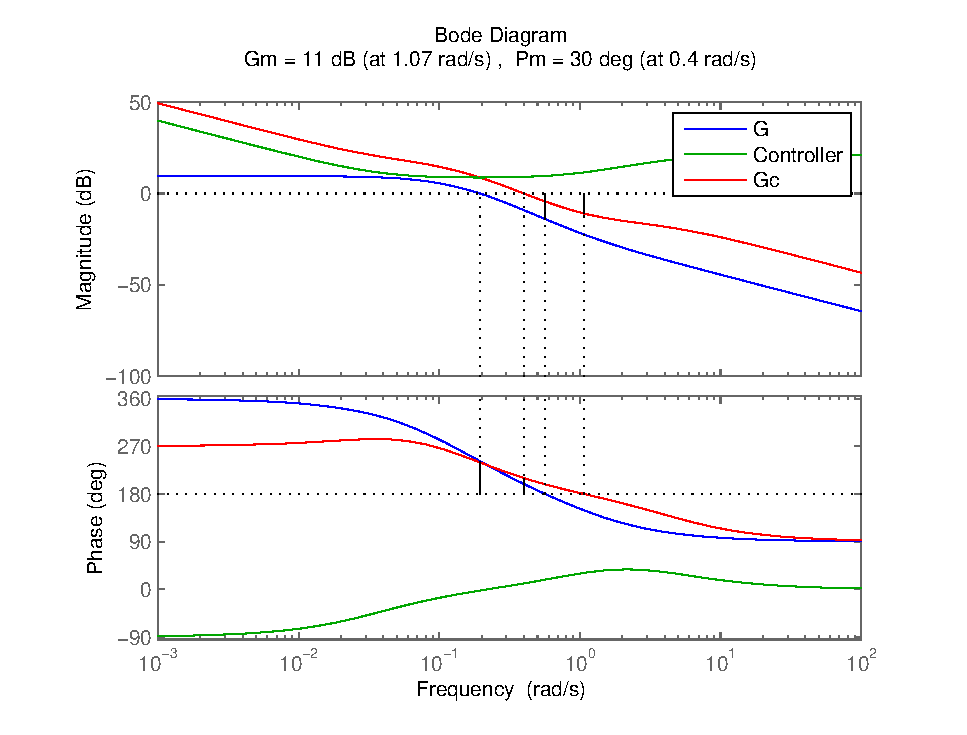
\includegraphics[width=\columnwidth]{fig/bode411.eps}
    \caption{Bode diagram of the system's functions\\ Phase-margin: $30^{\circ}$} 
    \label{figbode411}
\end{figure}

\begin{figure}[h!b]
    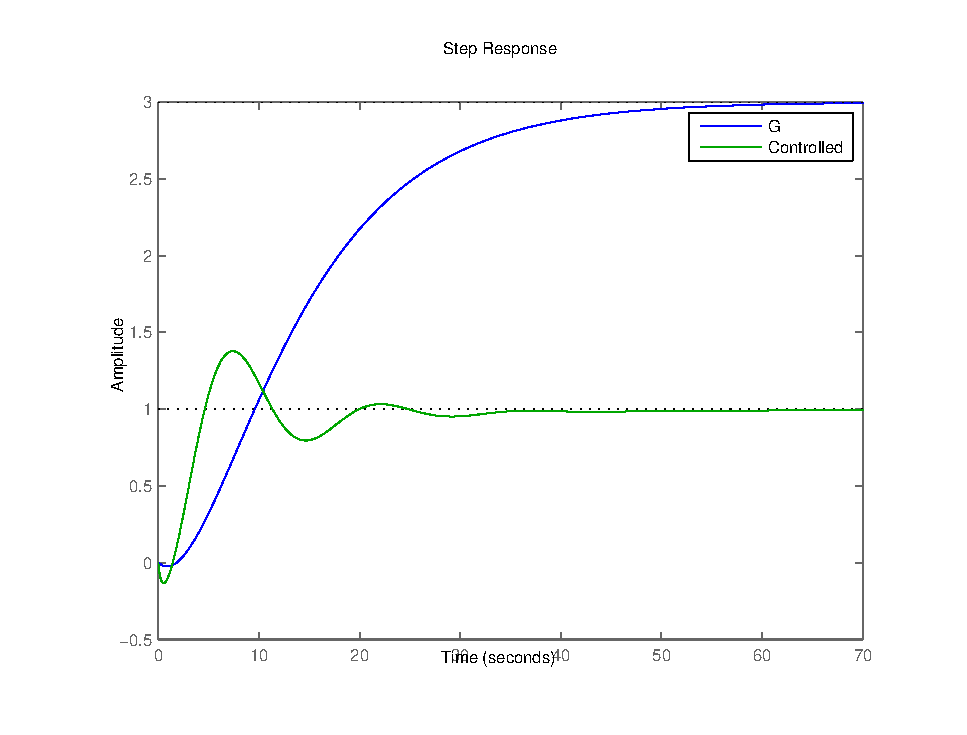
\includegraphics[width=\columnwidth]{fig/step411.eps}
    \caption{Step response of the system with and without the controller\\ Phase-margin: $30^{\circ}$}
    \label{figstep411}
\end{figure}



